\documentclass[paper=a4, fontsize=11pt]{scrartcl} % A4 paper and 11pt font size

\usepackage[T1]{fontenc} % Use 8-bit encoding that has 256 glyphs
\usepackage[english]{babel} % English language/hyphenation
\usepackage{amsmath,amsfonts,amsthm} % Math packages

\usepackage[skip=0pt]{caption}
\usepackage{subcaption}

\usepackage{lipsum} % Used for inserting dummy 'Lorem ipsum' text into the template
\usepackage{graphicx}
\usepackage{sectsty} % Allows customizing section commands
\allsectionsfont{\centering \normalfont\scshape} % Make all sections centered, the default font and small caps

\usepackage{fancyhdr} % Custom headers and footers
\pagestyle{fancyplain} % Makes all pages in the document conform to the custom headers and footers
\fancyhead{} % No page header - if you want one, create it in the same way as the footers below
\fancyfoot[L]{} % Empty left footer
\fancyfoot[C]{} % Empty center footer
\fancyfoot[R]{\thepage} % Page numbering for right footer
\renewcommand{\headrulewidth}{0pt} % Remove header underlines
\renewcommand{\footrulewidth}{0pt} % Remove footer underlines
\setlength{\headheight}{13.6pt} % Customize the height of the header

\iffalse
\numberwithin{equation}{section} % Number equations within sections (i.e. 1.1, 1.2, 2.1, 2.2 instead of 1, 2, 3, 4)
\numberwithin{figure}{section} % Number figures within sections (i.e. 1.1, 1.2, 2.1, 2.2 instead of 1, 2, 3, 4)
\numberwithin{table}{section} % Number tables within sections (i.e. 1.1, 1.2, 2.1, 2.2 instead of 1, 2, 3, 4)
\fi

\setlength\parindent{0pt} % Removes all indentation from paragraphs - comment this line for an assignment with lots of text

% new commands
\newcommand{\horrule}[1]{\rule{\linewidth}{#1}} % Create horizontal rule command with 1 argument of height

\title{	
\normalfont \normalsize 
\iffalse
\textsc{Massachusetts Institute of Technology \\ Sloan School of Management, Spring 2016} \\ [25pt] % Your university, school and/or department name(s)
\fi
\horrule{0.5pt} \\[0.4cm] % Thin top horizontal rule
\huge 14.273 Industrial Organization: Pset4 \\ % The assignment title
\horrule{.5pt} \\[0.4cm] % Thick bottom horizontal rule
}

\author{Dave Holtz, Jeremy Yang} % Your name

\date{\normalsize\today} % Today's date or a custom date

\begin{document}
\maketitle
\begin{itemize}
\item[1.] Model setup.\\

Following the notations in Rust (1987), HZ's flow utility is:
\[u(x_t,i_t,\theta_1)+\epsilon_t(i_t) = 
\begin{cases}
-RC-c(0,\theta_1)+\epsilon_t(1) & i_t = 1\\
-c(x_t,\theta_1)+\epsilon_t(0) & i_t=0
\end{cases}\]
where $RC$ is the replacement cost, $x_t$ is the observed state variable for mileage, $c(\cdot)$ is cost function and $i_t$ is the decision to replace engine and $\epsilon_t(\cdot)$ is action specific and type I extreme value distributed structural error (or unobserved state variable).\\

The state transition probability is given by:
\[\theta_{3j} = \mathbb{P}(x_{t+1}=x_t+j|x_t,i_t=0)\]
$j \in \{0,1,2\}$ and if $i_{t}=1$ then $x_{t+1}=0$ with probability 1.\\

HZ chooses $i_t$ in every period $t$ to maximize an infinite sum of discounted flow utilities. The maximal value is defined as the value function (suppress the dependency on $\theta_1, \theta_3$):
\[V(x_1,\epsilon_1) := \text{max}_{i_t, t\in\{1,2,..\}}\ \mathbb{E}[\sum_{t=1}^\infty \beta^{t-1} (u(x_t,i_t,\theta_1)+\epsilon_t(i_t))]\]

Rewrite the value function as in the Bellman optimality form:
\[V(x_t, \epsilon_t) = \text{max}_{i_t} \ (u(x_t,i_t,\theta_1)+\epsilon_t(i_t)) + \beta \mathbb{E}[V(x_{t+1},\epsilon_{t+1})|x_t, i_t]\]
where the expectation is with respect to (conditional) state transition probability of both $x$ and $\epsilon$, see Rust (1987) equation (4.5). The Bellman equation breaks the dynamic optimization problem into an infinite series of static choices. 


\item[2.]
\begin{itemize}
\item[(1)] The choice specific value function can be derived by plugging a specific action into the value function:
\[\tilde{V}(x_t,\epsilon_t,i_t)=
\begin{cases}
-RC-c(0,\theta_1)+\epsilon_t(1) + \beta \mathbb{E}[V(x_{t+1},\epsilon_{t+1})|x_t, i_t=1] \\
-c(x_t,\theta_1)+\epsilon_t(0) + \beta \mathbb{E}[V(x_{t+1},\epsilon_{t+1})|x_t, i_t=0]
\end{cases}\]
\[V(x_t,\epsilon_t) = \text{max}\{\tilde{V}(x_t,\epsilon_t,1),\tilde{V}(x_t,\epsilon_t,0)\}\]
HZ's decision is about trading off the total (future) cost of maintaining an old engine and the lump sum cost of replacing to a new one. The time to replace is the stopping time in this problem, so it can be thought as an optimal stopping time problem where the optimal policy is characterized by a cutoff in $x$, HZ would choose to replace the engine if $x$ is above that threshold (the threshold depends on realized value of $\epsilon$).

\item[(2)] It's clear from 2 (1) that the optimal stopping rule is: 
\begin{align*}
&-RC-c(0,\theta_1)+\epsilon_t(1) + \beta \mathbb{E}[V(x_{t+1},\epsilon_{t+1})|x_t, i_t=1] >\\
&-c(x_t,\theta_1)+\epsilon_t(0) + \beta \mathbb{E}[V(x_{t+1},\epsilon_{t+1})|x_t, i_t=0]
\end{align*}
or, 
\[\tilde{V}(x_t,\epsilon_t,1) > \tilde{V}(x_t,\epsilon_t,0)\]
therefore, because the errors are type I extreme value distributed:
\[\mathbb{P}(i_t=1|x_t) = \frac{\text{exp}(u(x_t,1,\theta_1)+\beta \mathbb{E}[V_{t+1}|x_t, i_t=1])}{\sum_{k=\{0,1\}}\text{exp}(u(x_t,k,\theta_1)+\beta \mathbb{E}[V_{t+1}|x_t, i_t=k]}\tag{2.1}\]
where $u(x_t,i_t,\theta_1)$ is defined in 1 and for convenience:
\[V_{t+1} :=V(x_{t+1},\epsilon_{t+1})\]

\item[(3)]
For discrete $x$, under the assumption that the errors are type I extreme value distributed, we have (Rust (1987) equation (4.14)):
\[EV(x,i) = \sum_y \text{log} \{\sum_{j} \text{exp}[u(y,j)+\beta EV(y,j)]\}\cdot p(y|x,i)\tag{2.2}\]
where 
\[EV(x,i) := \mathbb{E}[V_{t+1}|x_t,i_t]\] 
and $x, i$ are the state and choice of current period and $y,j$ are the state and choice of the next period. Also note that here the transition probability does not depend on $x_t$ but only on $j$ (or $\Delta x$). To compute expected value function, we first need to estimate transition probability from the data, this can be done simply by counting:
\[\hat{\theta}_{30} = \frac{\sum_{b}\sum_{t} 1_{\{x_{bt+1}-x_{bt}=0, i_{bt}=0\}}}{\sum_{b}\sum_{t} 1_{\{i_{bt}=0\}}}\]
\[\hat{\theta}_{31} = \frac{\sum_{b}\sum_{t} 1_{\{x_{bt+1}-x_{bt}=1, i_{bt}=0\}}}{\sum_{b}\sum_{t} 1_{\{i_{bt}=0\}}}\]
\[\hat{\theta}_{32} = \frac{\sum_{b}\sum_{t} 1_{\{x_{bt+1}-x_{bt}=2, i_{bt}=0\}}}{\sum_{b}\sum_{t} 1_{\{i_{bt}=0\}}}\]
we compute the expected value function in the inner loop of the nested fixed point algorithm (holding the value of $\theta$ fixed), we first guess the initial values of $EV(x,i)$ for all possible values of $x,i$ and use the equation (2.2) to iterate expected value function until it converges. The criterion is:
\[\text{max}_{x,i}|EV^{T+1}(x,i)-EV^T(x,i)|<\eta\]

The plot for $x=1-30$ at the true value of parameters are shown below:

\begin{figure}[ht!]
\centering
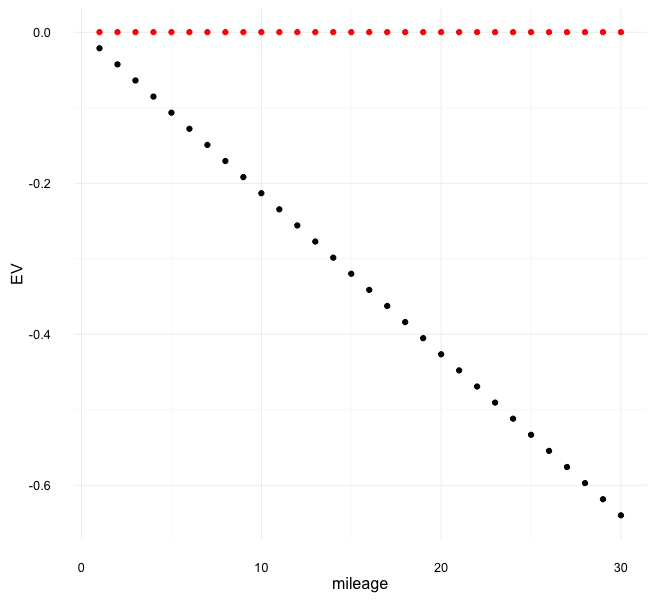
\includegraphics[scale=.6]{EV.png}
\caption{Expected Value Function (black for $i=0$ and red for $i=1$)} 
\end{figure} 

\item[(4)]
Summary statistics.

\end{itemize}

\item[3.]
\begin{itemize}
\item[(1)] In the outer loop we search over a grid of values for $(\theta_1, \beta, RC)$, and compute the log likelihood function:
\[\text{log}L = \sum_{b} \{\sum_{t} \text{log} \mathbb{P}(i_{bt}|x_{bt}) + \sum_t \text{log} \mathbb{P}(x_{bt}|x_{bt-1},i_{t-1})\}\]
where $b$ indexes for bus and $t$ indexes for time period. We compute a log likelihood for each combination of values for $(\theta_1, \beta, RC)$ and choose the one that has the maximal value as our maximum likelihood estimation.
\end{itemize}

\end{itemize}

\end{document}